\documentclass[i2]{oss}
\usepackage[english]{babel}
\usepackage{graphicx}

\usepackage{fullpage}
\usepackage{color}
\usepackage{soul}
%\usepackage{gensymb}
\usepackage{caption}
\usepackage{subcaption}
\usepackage[section]{placeins}
\usepackage{titlesec}
\usepackage{wrapfig}
\usepackage{color}
% Automatically introduces paragraph spacing
\usepackage{parskip}

% Lets Latex correctly interpret the symbols: < >
\usepackage[T1]{fontenc}

\setcounter{secnumdepth}{4}
\titleformat{\paragraph}
{\normalfont\normalsize\bfseries}{\theparagraph}{1em}{}
\titlespacing*{\paragraph}
{0pt}{3.25ex plus 1ex minus .2ex}{1.5ex plus .2ex}

\newcommand{\class}[1]{\texttt{#1}}
\newcommand{\method}[1]{\texttt{#1}}
\newcommand{\junit}{\emph{JUnit }}
\newcommand{\Daemon}{\class{Daemon  }}
\newcommand{\gloss}[1]{\textbf{#1}}
\newcommand{\col}[1]{\textcolor{red}{#1}}
\newcommand{\comment}[1]{{\huge \textcolor{green}{#1}}\\}

\begin{document}

\members{Joren Verspeurt {\small \texttt{(r0258417)} } \\ %# Commentaar
         Sophie Marien {\small \texttt{(s0216517)}}\\
         Stef Noten {\small \texttt{(s0211264)}}\\
         Toon Nolten {\small \texttt{(r0258654)}} \\
         Begeleider: Mario H. C. T.} % teamleden

\maketitlepage
\newpage
\tableofcontents
\pagebreak




%-----------------------------------------------------------------------
%	INLEIDING
%-----------------------------------------------------------------------
\section*{Introduction}
\label{ssec:introduction}
%introductie en de belangrijkste elementen van ons ontwerp
In the first iteration we assessed the design and implementation of \junit and in the second iteration we had to extend it with a daemon that would continuously test a given project according to a policy chosen by the user.
In this iteration we have to expand \junit with ...  

In the first section we discuss the implementation of the composition of the policies. 
After that the design is explained.
In section 3... the refactoring and the .. are discussed. 
At the end we discuss the project and give an evaluation.


\section{Extension}

For the third iteration we have to extend the functionality of the policies. 
It should be possible to combine multiple policies. This would mean that every policy regularly can decide which test will follow and that no policy always takes precedence over the other policies.\\

In our implementation all the policies will set an order to their tests. All these list with test that have an order provided by the policy will be merged with each other. The merging will be as follow: 
\begin{itemize}
\item First it will take one Policy and take the first test in the list and put this test as first.
\item Second it will look in the other lists of tests of the other policies if this test is in the list. If this test is an element of the list it will be discarded. 
\item Third the second Policy will say which test it will be given.
\item Again we will check in the other lists if this test is in the list.
\item This will go on until no tests are left in the lists.
\end{itemize}

Instead of that we will see what the order is of the tests we will ask the Policies which order they want to give to the test. We will do this because if a Policy has no data for a test it can not give an order to this test. If it cannot give an order to a test it is no use to let this policy decide when this test will be set. 


\begin{table}[h!]
\begin{center}
    \begin{tabular}{ c  c  c  c | c}
     Policy 1 & Policy 2 & Policy 3 & Policy 4 & Order  \\ \hline
    	A & B & A & E & A \\
        B & D & B & D & B \\
        C & E & C & G & C\\
        D & G & F & \col{I'} & E \\
        E & F & J & \col{H'} & D \\
        F & \col{A'} & \col{G'} & \col{B'} & G \\
        G & \col{C'} & \col{H'} & \col{A'} & F \\
        H & \col{I'} & \col{D'} & \col{J'} & J \\
        \col{I'} & \col{J'} & \col{E'} & \col{C'} & H \\
        \col{J'} & \col{H'} & \col{J'} & \col{F'} & \col{I'} \\
    \end{tabular}
    \caption{Example of merging of policies }
    \label{fig:orderex}
    \end{center}
\end{table}

Figure \ref{fig:orderex} gives an example of the merging of the policies. The test are A to I. If a policy has no data about a test and can thus not give an order to the test it is marked with an accent ('). 


\subsection{Design}

Use of composite. 

The order of the tests of multiple policies has to be fair. The first choise was to give every tests a weight according to the order the policy gives to the test. 


Every Policy will give a weight to the tests. If we use a lineair weight scale for the test, ... 
Therefore we use another function for the weight, for example exponential. By doing this the tests in front will be more likely to be in the beginning and the last tests will be at the end. 

If the total weight of multiple tests are the same we use another method to put test first. .. Voorbeeld van in de opgave.

Volgorde kan niet uit een request en een sortable gehaald worden. 


\section{Analyse}
In this section we will analyse our project with the extention. 

%-----------------------------------------------------------------------
%	PROJECT MANAGMENT
%-----------------------------------------------------------------------
\section{Project management}
\label{ssec:Projectmanag}
%Een beschrijving van de taakverdeling voor elk teamlid: een concrete beschrijving van
%elke taak en activiteit en de tijd die hierin werd genvesteerd.
% Een schatting van de totale tijd die elk teamlid in dit project heeft genvesteerd

The division of tasks was about the same for everybody. Because it was a small task the design and the implementation was done together. In table \ref{tab:werkuren} the workhours per teammember can be seen for the different parts of the assignment. The different parts are various (setting up eclipse, visual paradigm, \junit, .. ), design, implementation and report. 



%TODO tekst


\begin{table}[h!]
\begin{center}
    \begin{tabular}{ r | c  c  c  c  c  c}
     & Joren & Toon & Stef & Sophie \\ \hline
    	Various & 		3u30 & 4u00 & 4u00 & 4u00\\
        Design & 		14u30 & 20u30 & 25u00 & 20u30 \\
        Implementation & 28u00 & 34u30 & 40u30 & 16u50\\
        Report & 		18u00 & 16u00 & 21u00 & 16u40 \\
        Total & 		00u00 & 00u00 & 00u30 & 00u00  
    \end{tabular}
    \caption{Overview of the workhours per subject}
    \label{tab:werkuren}
\end{center}
\end{table}

%TODO figuren updaten
\begin{figure}[h!]
        \centering
        \begin{subfigure}[hb]{0.20\textwidth}
                \centering
                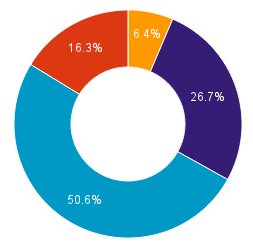
\includegraphics[width=\textwidth]{chart_2}
                \caption{Joren}
        \end{subfigure}%
        \begin{subfigure}[hb]{0.20\textwidth}
                \centering
                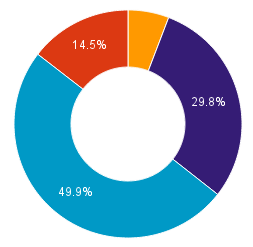
\includegraphics[width=\textwidth]{chart_3}
                \caption{Toon}
        \end{subfigure}%
        \begin{subfigure}[hb]{0.20\textwidth}
                \centering
                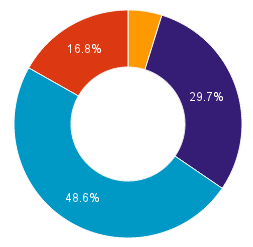
\includegraphics[width=\textwidth]{chart_4}
                \caption{Stef}
        \end{subfigure}%
        \begin{subfigure}[hb]{0.20\textwidth}
                \centering
                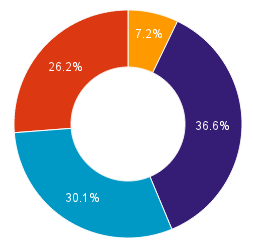
\includegraphics[width=\textwidth]{chart_5}
                \caption{Sophie}
        \end{subfigure}%
                \begin{subfigure}[hb]{0.20\textwidth}
                \centering
                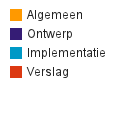
\includegraphics[width=\textwidth]{legende}
                \caption{Legend}
        \end{subfigure}%


 \caption{Overview of the division of tasks}
\label{fig:werkverdeling}
\end{figure}

 

\end{document}